\chapter{Fundamentals}
In this chapter, we embark on a journey to construct the narrative foundation that underpins our
thesis. Here, we will introduce the essential design concepts and the innovative technologies that
have been employed in the creation of the platform known as Kube. This platform is envisioned as an
ERP system that not only encapsulates the core functionalities typical of such software but also
adopts a serverless and microservice architecture. To achieve this, we will delve into the process
of fragmenting the ERP into smaller, more manageable modules. These modules will then be intricately
woven together and seamlessly integrated within a FaaS (Function as a Service) model environment,
exemplified by services such as AWS Lambda. This integration is key to realizing a system that is
both highly modular and scalable, leveraging the agility afforded by serverless computing and the
robustness of microservices. Through this exploration, we aim to provide a detailed understanding of
both the design philosophy and the technological framework that define the functionality and
innovation of Kube.

\section{Cloud Computing}
The advent of cloud computing has revolutionized the way we approach computing and data management.
This section of the thesis will explore the paradigm of cloud computing, which has emerged as a
transformative force in the technological landscape. We will examine the fundamental aspects of
cloud computing, including its service models, deployment strategies, and the pivotal role it plays
in modern IT infrastructure.

\subsection{Definition}
The United States National Institute of Standards and Technology's definition of cloud computing
is\textsuperscript{\cite{nist}}:

\begin{quote}
    Cloud computing is a model for enabling ubiquitous, convenient, on-demand network access to a
    shared pool of configurable computing resources (e.g., networks, servers, storage, applications, and
    services) that can be rapidly provisioned and released with minimal management effort or service
    provider interaction. This cloud model is composed of five essential characteristics, three service
    models, and four deployment models.
\end{quote}

Cloud computing offers a highly flexible service delivery model, enabling on-demand access to
various resources, such as storage, processing power, and applications, via the internet. This
eliminates the need for local servers, shifting data handling to online remote servers and offering
a cost-effective, pay-for-what-you-use pricing model. Services like Amazon Web Services (AWS)
provide the technology infrastructure, allowing users to scale operations with ease. Additionally,
this model promotes economic efficiency, as organizations pay only for resources they consume,
supporting a scalable and agile approach to resource management. The network, often the internet,
serves as a conduit between users and cloud services, ensuring data is managed with strong security
measures.

\subsubsection{Essential Characteristics}
Five essential characteristics of cloud computing are\textsuperscript{\cite{nist}}:
\begin{itemize}
    \item \textbf{On-Demand Self-Service}: Users can independently set up and manage their computing needs, such as
          server time and network storage, automatically, eliminating the need for direct interaction with
          service providers.
    \item \textbf{Broad Network Access}: Services are accessible over the internet using standard methods that
          support a diverse range of devices, including smartphones, tablets, laptops, and desktops.
    \item \textbf{Resource Pooling}: The provider's computing resources are aggregated to serve various customers
          under a multi-tenant model. Resources are dynamically allocated and reallocated based on user
          demand, with the user typically not knowing or controlling the exact physical location of the
          resources but may be able to designate a location at a broader level (such as country, state, or
          data center).
    \item \textbf{Rapid Elasticity}: Services can be quickly scaled up or down to match demand, with the scaling
          process sometimes occurring automatically. From the user's perspective, the supply of available
          resources often seems boundless and can be acquired in any volume at any time.
    \item \textbf{Measured Service}: Cloud platforms automatically monitor, control, and report resource usage with
          a metering function that operates at an appropriate level of detail, depending on the type of
          service, such as storage space, processing power, bandwidth, or active user numbers. This metering
          provides clear visibility into the usage of services for both the provider and the consumer.
\end{itemize}

\subsection{Service Models}
Cloud computing has revolutionized the way businesses approach technology, offering a spectrum of
services that cater to varying requirements for control, flexibility, and management. As
organizations transition to cloud-based solutions, understanding the different service models
becomes crucial for leveraging the full potential of the cloud.

The figure \ref{fig:3_cloud_models} shows the three primary cloud service models, forming what is
often referred to as the cloud computing "stack," include Infrastructure as a Service (IaaS),
Platform as a Service (PaaS), and Software as a Service (SaaS). These service models are designed to
build upon one another, offering layers of abstraction and increasing levels of managed
services\textsuperscript{\cite{cloud_amazon}}.

\begin{figure}
    \centering
    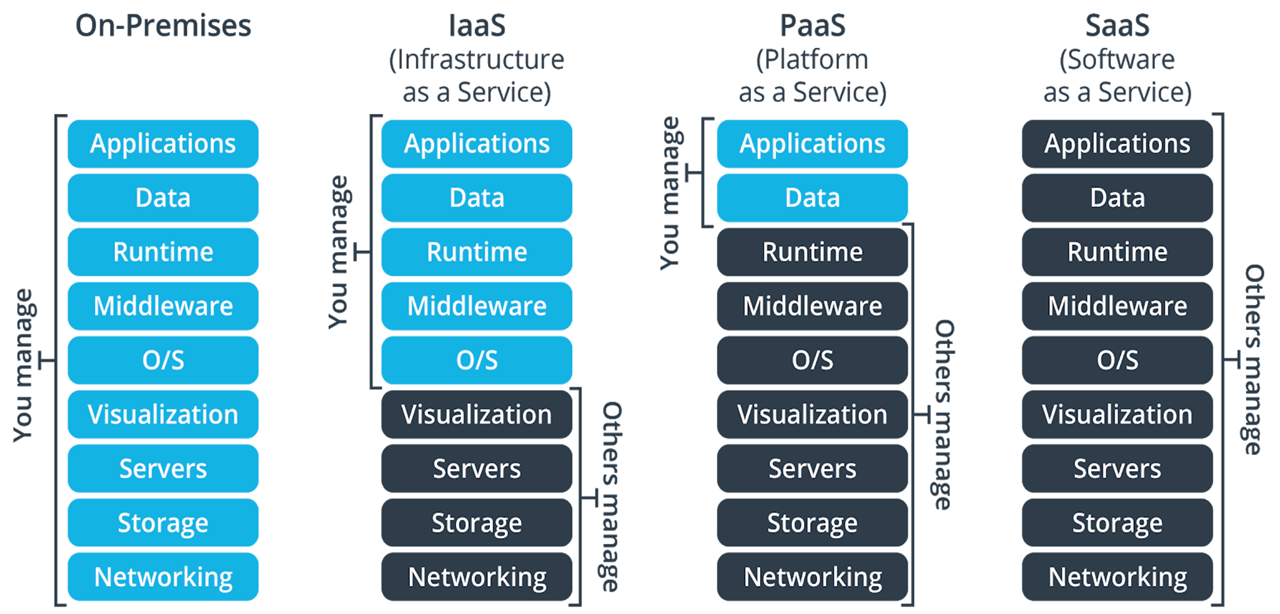
\includegraphics[scale=0.25]{Pictures/3_cloud_models.png}
    \caption{Cloud service models \textsuperscript{\cite{cloud_models}}.}
    \label{fig:3_cloud_models}
\end{figure}

\subsubsection{Infrastructure as a Service (IaaS)}
Infrastructure as a Service (IaaS) is a transformative approach to managing IT resources, offering
flexible and on-demand access to essential infrastructure services through the internet. This
includes virtual machines, storage, and networking that can be customized and billed based on actual
usage. IaaS grants organizations unprecedented control over their IT resources, closely resembling
traditional on-premises infrastructure. It allows for easy scalability without the need for costly
upfront investments in hardware. IaaS empowers consumers with the ability to provision processing,
storage, and networking resources, deploying and running various software, including operating
systems and applications. This level of customization enables organizations to tailor their IT
environment to their specific needs, ensuring a seamless and efficient operation in the cloud.

\subsubsection{Platform as a Service (PaaS)}
Platform as a Service (PaaS) is a significant innovation in cloud computing, offering comprehensive
hardware and software resources for cloud-based application development. Leading PaaS providers
simplify development by effectively managing the underlying infrastructure, allowing a laser focus
on application creation. With PaaS, you're free from infrastructure oversight, enabling dedicated
attention to application deployment and management, improving operational efficiency by eliminating
resource provisioning, capacity planning, and maintenance. PaaS provides an environment for
building, testing, and managing software applications without the need to manage the underlying
cloud infrastructure. As a user, you control your applications and their hosting settings,
simplifying the development process by allowing you to focus solely on creating and deploying your
applications.

\subsubsection{Software as a Service (SaaS)}
Software as a Service (SaaS) is a cloud computing model that delivers software applications over the
internet on a subscription basis. In this approach, cloud providers manage and host the
applications, ensuring their availability, performance, and security. Well-known examples of SaaS
offerings include Google Workspace, Microsoft Office 365, and Salesforce. SaaS provides a complete
software solution over the internet, including the application and its underlying infrastructure,
which is fully maintained by the cloud service provider. This approach spares users from managing
the infrastructure, as the provider handles software updates and security measures. Users can access
these applications through different devices and web browsers, enjoying an accessible and simplified
experience. SaaS enables users to efficiently utilize applications hosted on the cloud, focusing
solely on using the software rather than its maintenance.

\subsection{Deployment Models}
% possibile immagine da qui https://www.slideteam.net/cloud-computing-deployment-models-cloud-service-models-it.html
Cloud computing, a key driver in modern IT resource management, offers various deployment models
tailored to different business needs, security requirements, and scalability demands. This
exploration focuses on Public, Private, Hybrid, and Community Cloud models, discussing their unique
features, benefits, and considerations.

\subsubsection{Community Cloud}
Community-dedicated cloud infrastructure is exclusively used by a specific community of
organizations with shared interests, including mission objectives, security requirements, policies,
and compliance regulations. This infrastructure can be managed by one or more organizations within
the community, external providers, or a combination of both, and it can be located on-premises or
off-premises to accommodate community preferences\textsuperscript{\cite{nist}}.

\subsubsection{Private Cloud}
A private cloud is a form of cloud computing providing exclusive resources and services via a
private network, dedicated solely to one organization. It offers enhanced security and data
isolation, with the ability to tailor infrastructure and software to specific needs and workflows.
While offering robust security and control, private clouds can be costlier due to the organization's
responsibility for infrastructure management and scaling. These can be deployed on-site or hosted by
third-party providers, catering specifically to businesses requiring high security and compliance
standards. The combination of cloud computing benefits with heightened data security and
customization makes private clouds an attractive option for businesses handling sensitive data.

\subsubsection{Public Cloud}
In public cloud computing, a third-party service provider manages all the level of infrastructure,
including servers, storage, and computing resources. Clients access these resources via the internet
and are billed based on their actual usage, creating a cost-effective and flexible pay-as-you-go
model. These cloud environments eliminate the need for substantial investments in expensive
infrastructure, democratizing access to cloud computing. It's important to note that public clouds
operate on shared infrastructure, which offers cost efficiencies but raises concerns about data
isolation and privacy, as multiple customers' data and applications coexist on the same
infrastructure.

\begin{figure}
    \centering
    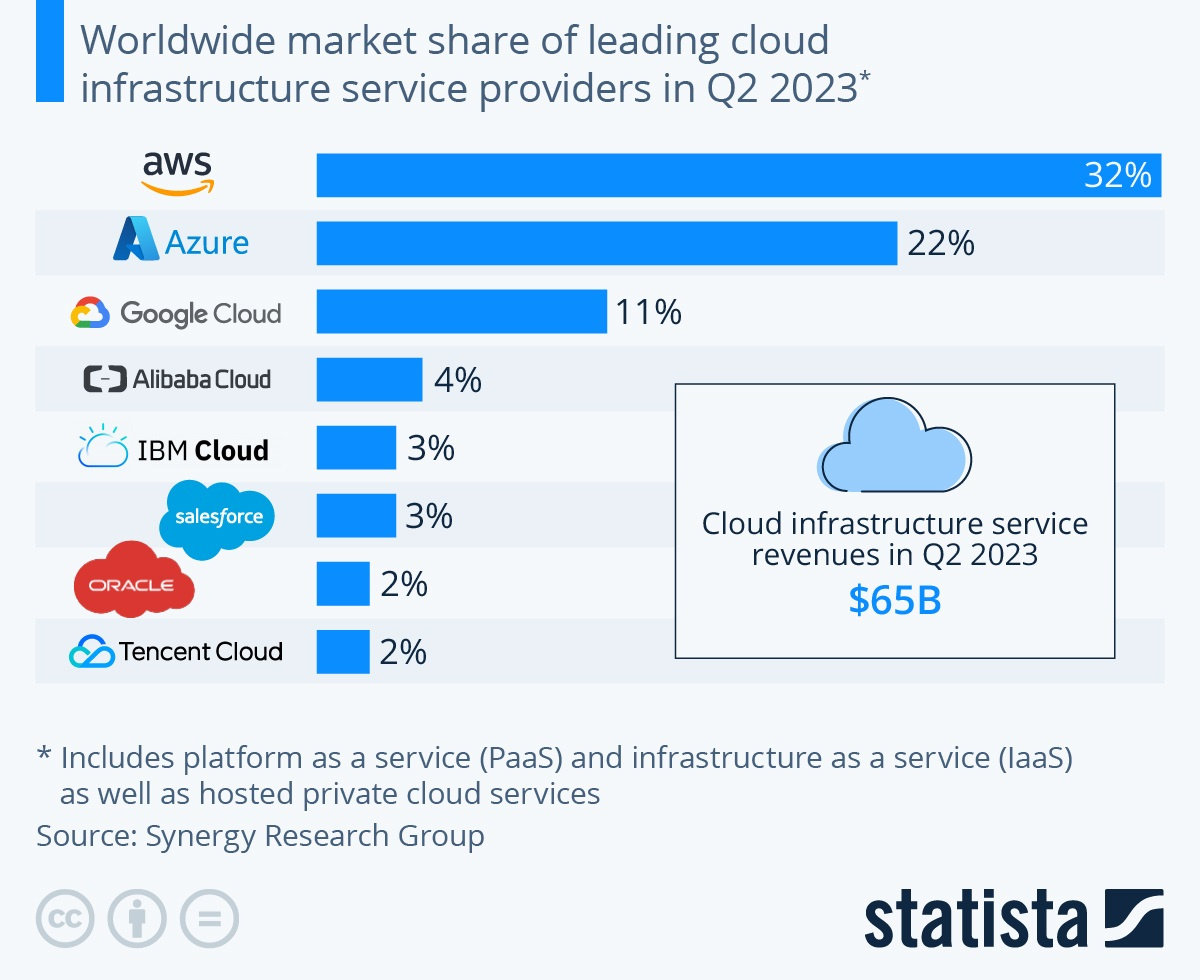
\includegraphics[scale=0.25]{Pictures/3_cloud_vendors.png}
    \caption{Worldwide market share of leading cloud infrastructure service providers in Q2 2023\textsuperscript{\cite{market_cloud_vendors}}.}
    \label{fig:3_cloud_vendors}
\end{figure}

The figure \ref{fig:3_cloud_vendors} show how the public cloud marketplace consists of numerous
cloud providers. Amazon, Microsoft and Google account for 65\% of the total 2023 cloud market. The
remaining public cloud market is divided among IBM, Alibaba, Oracle and several smaller players. The
table \ref{tab:cloud_providers} make a comparison between the major cloud providers.

\begin{table}
    \centering
    \begin{tabular}{|l|c|p{3.8cm}|p{3.8cm}|}
        \hline
        \textbf{Name}            & \textbf{Cost/hour} & \textbf{Pros}                              & \textbf{Cons}                                            \\ \hline
        \textbf{Amazon AWS}      & \$0.0255           & Reliability, Quality, Professional Support & Expensive despite regular lowering of price              \\ \hline
        \textbf{Google GCP}      & \$0.0475           & Reliability, Affordable                    & Limited features and services                            \\ \hline
        \textbf{Microsoft Azure} & \$0.043            & Best infrastructure configuration          & Unsatisfactory customer experience and technical support \\ \hline
        \textbf{IBM Cloud}       & \$0.04             & Flexibility, Speed, Interoperability       & Complicated pricing model and platform can be slow       \\ \hline
    \end{tabular}
    \caption{Comparative overview of major cloud service providers\textsuperscript{\cite{top_cloud_vendors}}.}
    \label{tab:cloud_providers}
\end{table}

\subsubsection{Hybrid Cloud}
The hybrid cloud is an advanced cloud computing model that blends public and private clouds, giving
organizations the flexibility to distribute their applications and workloads as needed. This setup
allows for greater control and scalability than using only public clouds, letting businesses keep
sensitive data secure while still enjoying public cloud efficiency. It's ideal for companies that
need both strong security and the ability to quickly adapt and scale. The hybrid cloud offers a
versatile IT infrastructure that adjusts to the complex needs of modern businesses, improving
security, compliance, and overall efficiency. This makes it a valuable asset for companies
navigating the rapidly changing digital world.

\subsection{Benefits}
Cloud computing is a big shift from the traditional way businesses think about IT resources. Here
are seven common reasons organizations are turning to cloud computing services\textsuperscript{\cite{cloud_azure}}:

\begin{itemize}
    \item \textbf{Cost}: Cloud computing reduces the capital expense of buying hardware and
          software, setting up and running on-site datacenters, which can quickly add up.
    \item \textbf{Speed}: Cloud services are typically on-demand, allowing vast amounts of computing
          resources to be provisioned in minutes, offering businesses flexibility and easing capacity
          planning.
    \item \textbf{Global Scale}: It includes the ability to elastically scale IT resources,
          providing the right amount of computing power, storage, and bandwidth when and where needed.
    \item \textbf{Productivity}: Cloud computing eliminates many time-consuming tasks associated
          with managing on-site datacenters, allowing IT teams to focus on more important business goals.
    \item \textbf{Performance}: Cloud services run on a worldwide network of secure datacenters,
          regularly upgraded to the latest generation of fast and efficient computing hardware, offering
          benefits like reduced network latency and greater economies of scale.
    \item \textbf{Reliability}: Data backup, disaster recovery, and business continuity are easier
          and less costly, as data can be mirrored at multiple redundant sites on the cloud provider’s
          network.
    \item \textbf{Security}: Cloud providers typically offer a broad set of policies, technologies,
          and controls to strengthen security, protecting data, apps, and infrastructure from threats.
\end{itemize}

\subsection{Market Overview}
The global cloud computing market, valued at USD 483.98 billion in 2022, is expected to exhibit a
robust compound annual growth rate (CAGR) of 14.1\% from 2023 to
2030\textsuperscript{\cite{market_cloud_computing}}. This remarkable growth is attributed to the
cloud's capacity to significantly enhance business performance in large enterprises, the increasing
demand for hybrid and Omni-cloud systems, and the adoption of pay-as-you-go models. Cloud services
have gained popularity in developing countries, thanks in part to government initiatives aimed at
safeguarding data integrity and security. The COVID-19 pandemic has expedited the adoption of cloud
computing, driven by the shift towards hybrid work models. While data privacy and security concerns
remain, large enterprises are increasingly turning to cloud-based technologies to optimize costs.
Moreover, cloud adoption is on the rise among small and medium-sized organizations, and governments
in developing nations are making substantial investments in cloud delivery models to enhance
productivity. The Figure \ref{fig:3_cloud_computing_market} illustrates the growth of the U.S. cloud
computing market.

\begin{figure}
    \centering
    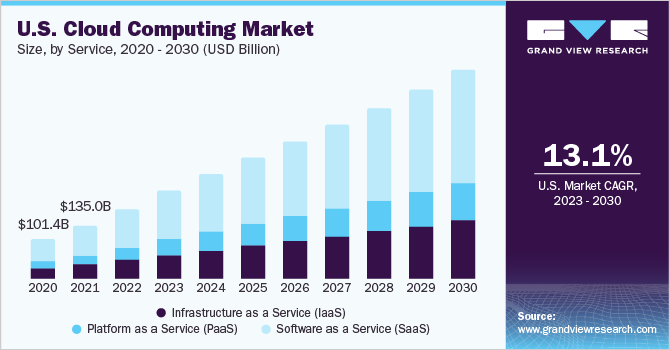
\includegraphics[scale=0.5]{Pictures/3_cloud_computing_market.png}
    \caption{U.S. cloud computing market\textsuperscript{\cite{market_cloud_computing}}.}
    \label{fig:3_cloud_computing_market}
\end{figure}

\section{Microservices}
This section of the thesis is dedicated to a comprehensive exploration of microservices as an
architectural choice that has seen an increasingly popularity over the past half-decade. It aims to
unpack the intricacies of microservices, given a broad overview of the core ideas behind this technology and some
reasons why these architectures are used so widely.

\subsection{Characteristics}
Microservices architecture is a modular approach to software development, breaking complex
applications into smaller, independent components—microservices—tailored to specific business
domains like inventory management or order processing. These microservices, with well-defined
interfaces, can be developed and deployed independently, ensuring flexibility and the evolution of
each component without affecting others. This architecture supports a service-oriented approach,
emphasizing independent deployability and technology neutrality, suitable for diverse technical
challenges\textsuperscript{\cite{microservices_book}}.
\newline\newline
Internally, microservices encapsulate their functionality, operating via network endpoints and
hiding implementation details like programming languages or data storage. This ensures effective
complexity management, with each service maintaining its own data storage, avoiding shared database
issues.
\newline\newline
Externally, microservices act as 'black boxes,' offering functionality without exposing internal
processes. This approach protects against impacts from internal changes, as long as interfaces
remain compatible. It enables seamless updates and maintenance, supporting independent development
and continuous integration.
\newline\newline
Key characteristics of microservices include loose coupling for flexibility and high cohesion for
maintainability. They allow targeted scalability, parallel team work, and robust security, with each
service secured separately. This makes microservices ideal for creating adaptable, scalable, and
sustainable software in rapidly evolving business and technology environments.

\subsubsection{Microservices in the Context of Cloud Computing}
The integration of microservices and cloud computing marks a significant progression in software
architecture, fostering dynamic, scalable, and resilient systems. The decentralized nature of
microservices aligns seamlessly with cloud environments, providing agility and scalable
infrastructure to meet varying service demands. Cloud platforms enhance resource optimization,
ensuring efficient and cost-effective operations. This synergy enables organizations to exploit
cloud computing's robustness, supporting microservices' complex interactions for heightened
scalability and resilience. It allows for continuous integration and deployment, promoting rapid
innovation. Additionally, strategic distribution of microservices across various regions in the
cloud enhances fault tolerance and ensures a consistent user experience globally.

\subsubsection{Example of a Microservice Architecture}
A prime example of microservices in action is the streaming giant Netflix, which has become
synonymous with the successful implementation of this architectural style. The backend architecture
of Netflix, a detailed account of which is provided in an article on
DEV.to\textsuperscript{\cite{microservice_example}}, is a testament to the company's innovative
engineering approach.

\begin{figure}
    \centering
    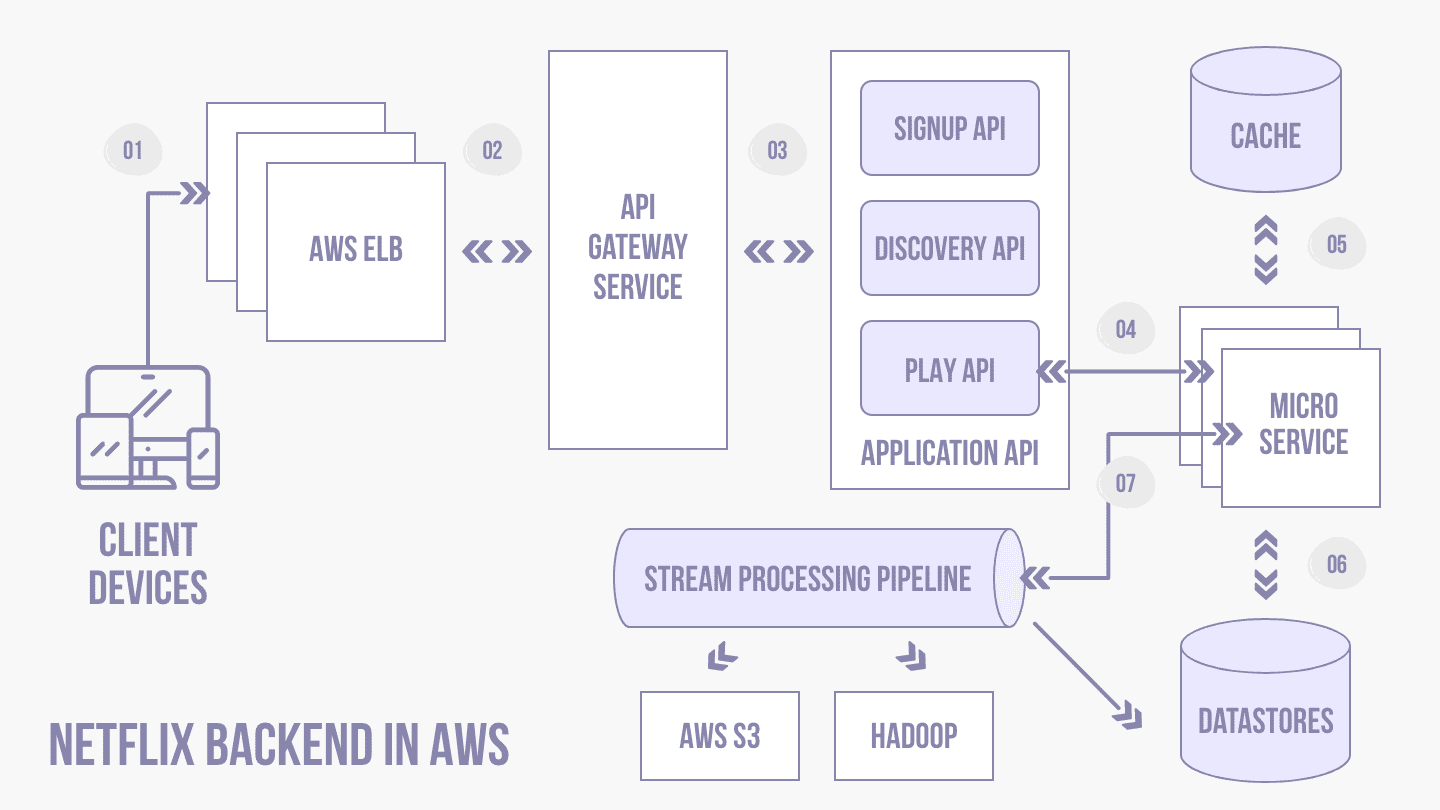
\includegraphics[scale=0.25]{Pictures/3_netflix.png}
    \caption{Netflix backend in AWS\textsuperscript{\cite{microservice_example_image}}.}
    \label{fig:3_netflix}
\end{figure}

How we can see in Figure \ref{fig:3_netflix}, Netflix's backend is a conglomeration of microservices
that operate on Amazon Web Services (AWS), enabling them to serve a staggering amount of content
globally with high availability and resilience. Each microservice is designed to perform a specific
function, such as handling login requests, processing user recommendations, or managing customer
support interactions. This division of responsibilities allows for independent scaling and
development of services, which is crucial given the diversity of Netflix's content and the
variability in demand. The microservices architecture is not only a core component of their backend
system but also underpins their Open Connect content delivery network (CDN), ensuring optimal
streaming performance by placing servers within Internet Service Provider (ISP) networks around the
world. This architecture facilitates rapid and reliable delivery of complex applications at scale,
illustrating the microservices model's capacity to support large-scale enterprise systems
efficiently and effectively.

\newpage

\subsection{Benefits}
This section delves into the multifaceted advantages of adopting microservices. From enhanced
scalability to independent deployment cycles, microservices promise a range of benefits that cater
to both technical and business needs. By dissecting these advantages, this section aims to elucidate
why microservices are becoming the architectural choice for many modern enterprises, providing them
with the flexibility and agility required to thrive in a competitive
market\textsuperscript{\cite{microservices_gitlab}}.

\subsubsection{Scalability}
Microservices excel in scalability due to their ability to be scaled individually. This granular
scalability allows for precise allocation of resources to different components based on fluctuating
demands, leading to enhanced efficiency in resource utilization. Unlike monolithic architectures,
where scaling often requires scaling the entire application, microservices operate independently.
This independence facilitates the seamless addition, removal, updating, or scaling of each service
without causing interruptions to the rest of the system. Organizations benefit from this by being
able to dynamically allocate resources to microservices experiencing spikes in demand—such as during
peak shopping seasons—and similarly, scale them down when demand wanes, thereby optimizing the use
of resources and computing power across the service landscape.

\subsubsection{Robustness}
Microservices architecture enhances the robustness of software applications by leveraging its
inherent decoupling. Individual services can fail without precipitating a system-wide shutdown,
thereby preventing a single point of failure from causing cascading breakdowns. In comparison,
monolithic architectures are susceptible to the domino effect, where a single component's failure
can paralyze the whole application. Microservices inherently design for failure, allowing the system
to degrade gracefully and maintain functionality even when certain services are down. However,
network and machine failures are inevitable, and strategies must be in place to handle these
incidents without significantly affecting the user experience.

\subsubsection{Technology agnostic}
Microservices architecture stands out for its technological flexibility, granting teams the liberty
to select the most suitable technology stack for each distinct service. This technology-agnostic
approach decouples services from any singular, early-stage technology decisions that often constrain
entire projects. Within this paradigm, each microservice can be developed using different
programming languages and data storage solutions, according to what best serves its purpose. This
not only streamlines development by aligning with teams' existing proficiencies but also avoids the
overhead of learning new languages unnecessarily. For instance, organizations like Netflix and
Twitter predominantly utilize the Java Virtual Machine (JVM) as their operational platform
\textsuperscript{\cite{microservices_book}}. Their choice is driven by a deep familiarity with this
technology.

\subsubsection{Distributed Development}
Microservices architecture allows development teams to independently build, deploy, and manage their
services, speeding up updates and feature additions with minimal disruption to the overall system.
This facilitates swift adaptation to changing business needs. Unlike monolithic applications, which
require large-scale deployments for minor updates, microservices support targeted, independent
changes to specific services. This reduces deployment risks, enables quick error recovery, and
hastens the delivery of new features to customers. Companies like Amazon and Netflix leverage
microservices to bypass obstacles in software delivery, ensuring rapid and reliable service to their
users\textsuperscript{\cite{microservices_book}}.

\subsubsection{Team optimization}
Microservices architecture enhances team productivity by adhering to the "two-pizza rule," where
smaller teams—ideally just large enough to be fed with two pizzas—tend to produce higher quality
outcomes due to improved focus and manageability. This approach, pioneered by Amazon, ensures that
each team works on a discrete codebase, fostering efficiency and faster achievement of goals. The
flexibility inherent in microservices also allows for easy reassignment of service ownership,
facilitating a seamless adaptation of the architecture to align with evolving organizational
structures, thereby maintaining efficiency and effectiveness in the long term.


\subsection{Challenges}
While the microservices architecture offers numerous benefits such as enhanced scalability and
improved team productivity, it also introduces a set of challenges that can complicate system design
and maintenance: the complexity of orchestrating numerous services, maintaining data consistency
across distributed systems and managing inter-service communication efficiently. Addressing these
challenges is essential for a smooth microservices architecture.

\subsubsection{Complexity}
The decentralized approach of microservices inherently leads to systems with a high degree of
complexity. As the number of services increases, the overall system can become more challenging to
oversee and manage. Debugging exemplifies this complexity; with each microservice generating its
logs, pinpointing the source of an issue can become a substantial challenge. This complexity
requires robust logging and monitoring solutions that can aggregate and correlate logs from across
services, providing a cohesive view of the system's health and facilitating faster problem
resolution. Additionally, the complexity demands that developers and operators have a clear
understanding of the system's architecture and communication patterns, ensuring they can effectively
trace and troubleshoot issues as they arise.

\subsubsection{Data Consistency}
Ensuring data consistency across microservices poses significant challenges due to their distributed
design. Unlike monolithic systems that rely on a single database, microservices often use separate
databases, making traditional transaction-based consistency difficult to maintain. As a result,
developers need to shift toward patterns like sagas and embrace eventual consistency, which can be a
major paradigm shift, especially when adapting existing systems. It's crucial to decompose
applications incrementally, allowing for careful evaluation of each change's impact on the system's
data integrity.

\subsubsection{Inter-service Communication}
In microservices architecture, especially in cloud environments, inter-service communication adds
complexity due to distributed network use. Each microservice's unique API requires careful
management to ensure compatibility, a significant task when hundreds or thousands of APIs are
involved. Disaggregating processes into multiple network-dependent services increases serialization,
transmission, and deserialization, potentially adding to latency. This impact on performance, hard
to predict in design or development, highlights the need for a gradual transition to microservices,
allowing for an assessment of changes on system latency.

\subsection{Comparison with Monolithic Architecture}

\begin{figure}
    \centering
    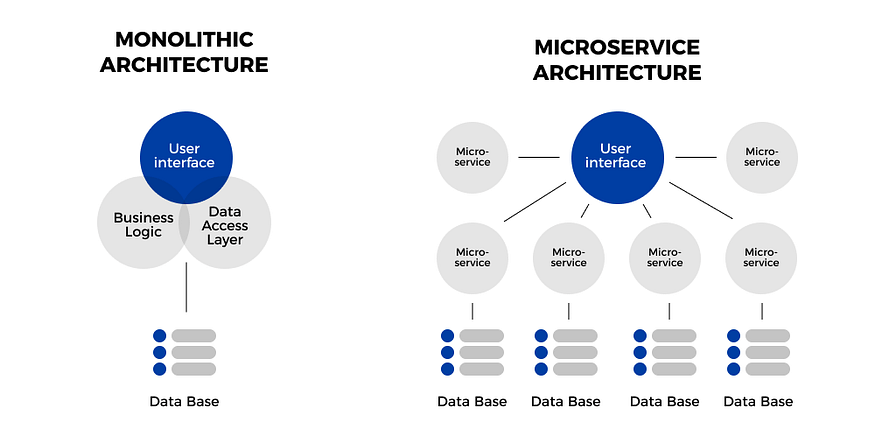
\includegraphics[scale=0.5]{Pictures/3_micro_mono.png}
    \caption{Monolithic and Microservices architectures\textsuperscript{\cite{monoliths_medium}}.}
    \label{fig:3_micro_mono}
\end{figure}

In Figure \ref{fig:3_micro_mono}, the distinction between a microservices approach and monolithic
architecture is illustrated. The latter is characterized by tightly coupled and interdependent
software components, any changes require building and deploying the entire stack, which can be slow
and error-prone. Microservices are designed to overcome these limitations by decomposing
functionality into separate services, each with a specific role, thus providing a more flexible and
scalable architecture. The table \ref{tab:micro_vs_mono} contains an overview of the differences
between the two approaches.

\begin{table}
    \centering
    \begin{tabular}{|l|p{5cm}|p{5cm}|}
        \hline
        \textbf{}            & \textbf{Monolithic}                                                                    & \textbf{Microservices}                                                       \\ \hline
        \textbf{Deployment}  & Simple and fast deployment of the entire system                                        & Requires distinct resources, making orchestrating the deployment complicated \\ \hline
        \textbf{Scalability} & It is hard to maintain and handle new changes; the whole system needs to be redeployed & Each element can be scaled independently without downtime                    \\ \hline
        \textbf{Agility}     & Not flexible and impossible to adopt new tech, languages, or frameworks                & Integrate with new technologies to solve business purposes                   \\ \hline
        \textbf{Resiliency}  & One bug or issue can affect the whole system                                           & A failure in one microservice does not affect other services                 \\ \hline
        \textbf{Testing}     & End-to-end testing                                                                     & Independent components need to be tested individually                        \\ \hline
        \textbf{Security}    & Communication within a single unit makes data processing secure                        & Interprocess communication requires API gateways raising security issues     \\ \hline
        \textbf{Development} & Impossible to distribute the team’s efforts due to the huge indivisible database       & A team of developers can work independently on each component                \\ \hline
    \end{tabular}
    \caption{Comparison of Monolithic and Microservices architectures\textsuperscript{\cite{monoliths_avenga}}.}
    \label{tab:micro_vs_mono}
\end{table}

\section{How to Model Microservices}
This section is dedicated to exploring key principles such as information hiding, coupling, and
cohesion, which are crucial in shaping our approach to defining the limits of our microservices. We
will place a particular focus on domain-driven design, a highly effective strategy that plays a
crucial role in establishing the boundaries of your microservices. This approach not only maximizes
their advantages but also effectively reduces potential risks.

\subsection{Boundaries}
Our goal is to design microservices that can be independently modified, deployed, and have their
features released to users without relying on others. The ability to update a single microservice
independently from the others is crucial. At their core, microservices represent a type of modular
decomposition, but with network interactions between modules. This means we can rely on a lot of
prior art in the space of modular software to assist in defining our boundaries. Bearing this in
mind, we will delve into three essential concepts crucial for identifying effective microservice
boundaries: information hiding, cohesion, and coupling\textsuperscript{\cite{microservices_book}}.

\subsubsection{Information Hiding}
Information hiding is a concept developed by David Parnas to look at the most effective way to
define module boundaries\textsuperscript{\cite{microservices_model_1}}. Information hiding aims to
conceal as much detail as possible within a microservice boundary. Parnas
write\textsuperscript{\cite{microservices_model_2}}:

\begin{quote}
    The connections between modules are the assumptions which the modules make about each other.
\end{quote}

Reducing assumptions between modules in microservices simplifies their connections, making it easier
to modify one module without affecting others. This approach also allows developers to make safer
changes, as they understand how their module is used by others, preventing the need for changes in
upstream components. Additionally, in microservices, such modifications can be deployed
independently, enhancing the benefits outlined by Parnas: faster development, better
comprehensibility, and increased flexibility.

% \begin{itemize}
%     \item \textbf{Improved development time}: Enabling independent development of modules
%           facilitates parallel work, thus diminishing the complexities often associated with increasing
%           the number of developers on a project.
%     \item \textbf{Comprehensibility}: The ability to examine and comprehend each module separately
%           simplifies the process of grasping the system’s overall functionality.
%     \item \textbf{Flexibility}: The independence of modules allows for alterations in one without
%           necessitating changes in others. Furthermore, this independence provides the flexibility to
%           recombine modules in various configurations, creating new functionalities.
% \end{itemize}

\subsubsection{Coupling and Cohesion}
The concepts of coupling and cohesion are integral to the structure and stability of microservice
architectures. Understanding their interplay helps in designing systems that are both stable and
efficient.
% Cohesion refers to how closely related the functionalities within a microservice are,
% aiming for a strong internal unity. Coupling, on the other hand, deals with the degree of
% interdependence between different microservices, where the goal is to minimize dependencies to
% achieve loose coupling. 
Achieving the right balance between these two aspects is crucial for the
effective functioning of microservices.

\begin{itemize}
    \item \textbf{Cohesion}: Cohesion in microservices is about strategically grouping related
          business functionalities to reduce the need for changes across multiple areas. It emphasizes
          consolidating similar behaviors in a single location, which streamlines the process of
          modification and deployment. This approach leads to strong cohesion, where closely related
          functionalities are contained within a single microservice, thereby enabling faster and more
          secure updates and changes.
    \item \textbf{Coupling}: Coupling in the context of microservices involves designing services in
          a way that changes in one do not require modifications in others. This design principle promotes
          minimal inter-service knowledge, thereby reducing dependencies between different services. The
          ideal state of loose coupling is achieved when services have minimal interactions with each
          other, maintaining their independence. This approach significantly reduces the risks associated
          with tightly interconnected systems, ensuring more robust and flexible service architecture.
\end{itemize}

This balance is not only about the technical aspects but also about making pragmatic decisions that
fit the specific context and challenges of the project.

\subsubsection{Types of Coupling}
The concept of coupling in system design is nuanced and not as straightforward as it might initially
appear. While it's true that excessive coupling can lead to various challenges in system
architecture, some level of coupling is inevitable and, in certain cases, necessary. The key
objective in effective system design is not to eliminate coupling entirely but to manage and
minimize its extent.

\begin{figure}
    \centering
    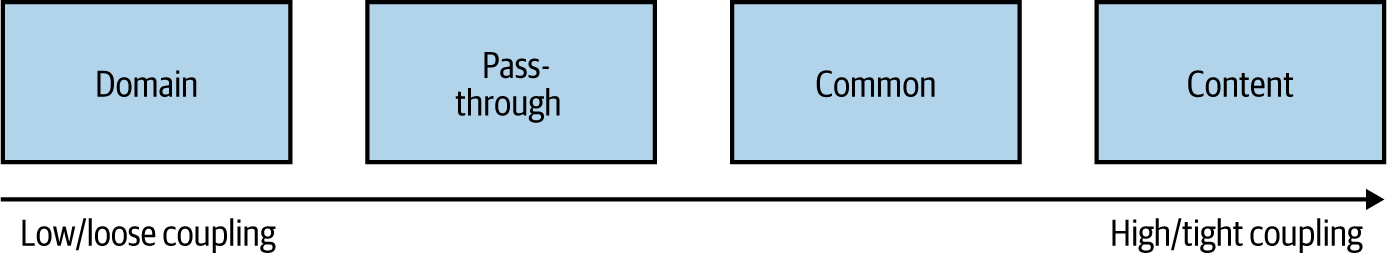
\includegraphics[scale=0.5]{Pictures/3_types_coupling.png}
    \caption{The different types of coupling, from loose (low) to tight (high)}.
    \label{fig:3_types_coupling}
\end{figure}

The different types of coupling\textsuperscript{\cite{microservices_book}}, as depicted in Figure
\ref{fig:3_types_coupling}, provide a comprehensive spectrum, ranging from low to high. Low coupling
is generally desirable as it indicates a system where components operate independently, enhancing
flexibility and ease of maintenance. High coupling, on the other hand, suggests a tightly
interlinked system where changes in one component can have significant ripple effects, making it
less desirable due to the increased complexity and risk involved. Understanding these variations and
their implications is crucial for designing robust, scalable, and maintainable systems.

\begin{itemize}
    \item \textbf{Domain Coupling}: Domain coupling refers to a scenario where one microservice
          depends on another for specific functionalities. While such interactions are largely inevitable
          in a microservice architecture, where collaboration among multiple services is essential for
          system operation, it's important to minimize these interactions. It is a form
          of loose coupling in microservices, but can lead to issues if a service relies too heavily on many
          downstream services, suggesting over-centralization of logic. Problems may also arise from
          exchanging complex data sets between services. It's advisable to share only essential
          information and minimize data exchange.
    \item \textbf{Pass-Through Coupling}: Pass-through coupling in microservices occurs when one
          microservice transmits data to another solely for the use of a subsequent downstream service.
          This form of coupling is particularly challenging within implementation strategies, as it
          suggests that the initiating service is aware not only of the direct recipient microservice but
          may also need to understand the functioning of the microservice further down the chain. This
          creates a complex interdependency where knowledge of multiple services and their interactions
          becomes necessary, complicating the architecture.
    \item \textbf{Common Coupling}: Common coupling in microservices refers to the scenario where
          multiple services utilize the same data set, such as a shared database, memory, or filesystem.
          This coupling becomes problematic when changes to the data's structure affect several services
          simultaneously. For example, if the schema of a commonly used database changes incompatibly, all
          services relying on it need updates. Additionally, common coupling can lead to resource
          contention issues, as multiple services accessing the same database or filesystem may strain or
          even incapacitate that resource. While sometimes manageable, common coupling often indicates a
          lack of cohesion in the system and can pose operational challenges, making it one of the less
          desirable forms of coupling.
    \item \textbf{Content Coupling}: Content coupling occurs when an upstream service intrusively
          modifies the internal state of a downstream service, commonly by directly accessing and altering
          the latter's database. This is subtly different from common coupling, where multiple services
          interact with a shared dataset, but acknowledge it as an external, uncontrollable dependency.
          Content coupling blurs ownership lines, complicating system modifications for developers. A
          clear distinction in microservices between changeable and unchangeable elements is crucial.
          Developers must be aware of the service contract exposed to external parties to avoid disrupting
          upstream consumers. While common coupling shares some issues with content coupling, the latter
          introduces additional complexities, often termed pathological coupling. Direct external access
          to a database challenges the definition of what can be safely altered and what cannot,
          undermining the principle of information hiding. Therefore, content coupling is best avoided due
          to these inherent complications.
\end{itemize}

% volendo puoi mettere le immagini

\subsection{Domain-Driven Design}
In defining microservice boundaries, we primarily focus on the domain itself, applying domain-driven
design (DDD) to model our domain more effectively. DDD, as introduced by Eric Evans in
"Domain-Driven Design"\textsuperscript{\cite{ddd_book}}, provides key concepts that are crucial in
this context. These include Ubiquitous Language, which ensures uniform language usage across the
domain; Aggregates, which group related domain objects into a single unit; and Bounded Context,
which sets the scope of applicability for a particular model. These principles play a vital role in
guiding our microservice architecture strategy.

\subsubsection{Ubiquitous Language}
Ubiquitous language emphasizes the importance of aligning the terminology in our code with the terms
used by the users. This commonality of language between the development team and the end users
simplifies modeling the real-world domain and enhances communication. Integrating real-world
language into the code streamlines the development process. It allows developers, when handling
tasks or stories, to quickly grasp the requirements and objectives, as these are expressed in terms
familiar to both the product owner and the development team.

\subsubsection{Aggregates}
Aggregates in microservice architecture are envisioned as self-contained units, each with its own
state, identity, and life cycle that mirrors real-world entities. These aggregates are apt for
implementation as state machines, given their inherent life cycles. The design focuses on
consolidating the code that manages state transitions with the aggregate's state itself. Typically,
a single microservice is responsible for one aggregate, but it may handle several. For instance, an
Invoice aggregate would include various line payments, each significant only within the context of
the overall Invoice aggregate.
\newline\newline
A microservice's role extends to managing the life cycle and data storage of one or several types of
aggregates. Should a different service need to modify an aggregate, it must either directly request
this change or prompt the aggregate to initiate its own state transitions, possibly in response to
events from other microservices. Aggregates are designed with the capability to reject inappropriate
state transition requests, underscoring the importance of preventing illegal state changes in their
implementation.

\subsubsection{Bounded Context}
A bounded context usually reflects a larger section of an organization, with clear responsibilities
within its boundaries. This concept focuses on concealing the finer details of implementation,
safeguarding internal aspects that aren't necessary for external understanding or involvement.
\newline\newline
In terms of structure, a bounded context comprises one or more aggregates. While some of these
aggregates might be visible externally, others remain internal to maintain the integrity of the
context. Bounded contexts can also form relationships with other contexts, translating into
dependencies between services in a microservice architecture.
\newline\newline
For instance, a warehouse service can be seen as a bounded context, bustling with activities like
processing outgoing orders, receiving new inventory, and other logistical tasks. In a different
bounded context, such as the finance department, the focus shifts to less dynamic but equally vital
functions like managing payroll and handling financial transactions. Each context operates within
its own realm of responsibilities but may interact with or depend on other contexts, reflecting the
interconnected nature of services in a microservices setup.

\subsubsection{Domain-Driven Design in Microservices}
Domain-Driven Design (DDD) is effective in microservices architecture due to its focus on bounded
contexts which conceal internal complexities and present clear boundaries to the system. These
contexts aid in maintaining stable microservice boundaries by ensuring that internal changes do not
affect other system parts. When systems are segmented along bounded contexts, modifications for
business needs are confined to specific microservices, streamlining deployment and reducing the
complexity of changes.

\newpage

\begin{figure}
    \centering
    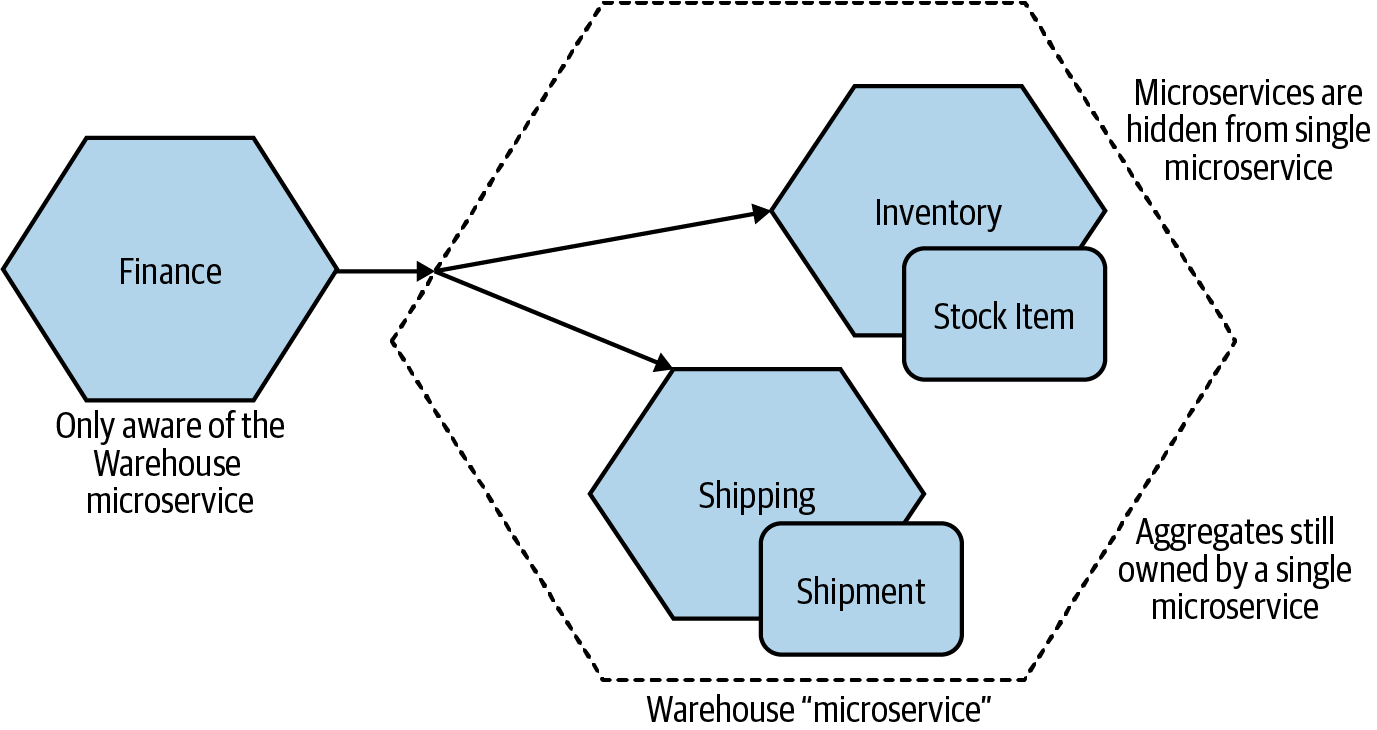
\includegraphics[scale=0.5]{Pictures/3_ddd.png}
    \caption{The Warehouse service internally has been split into Inventory and Shipping microservices}.
    \label{fig:3_ddd}
\end{figure}

Aggregates and bounded contexts both provide cohesive units with clear interfaces to the larger
system. Aggregates are focused state machines for single domain concepts, while bounded contexts
group these aggregates and represent them to the outside world. These constructs are ideal for
defining microservice boundaries. Initially, it's beneficial to work with services that cover
complete bounded contexts. If needed, services can later be divided into smaller ones without
splitting individual aggregates, keeping such internal decisions invisible to external stakeholders.
For instance, a Warehouse service may internally be divided into Inventory and Shipping, but
externally it remains a singular Warehouse microservice to users, as depicted in the figure
\ref{fig:3_ddd}.

\subsection{Coordination Management}
In the environment of microservices, the complexity of interactions extends beyond the simple
communication between two services. A critical aspect is the orchestration of multiple microservices
working together to execute comprehensive business processes. This orchestration requires a nuanced
approach to maintain the system's integrity and efficiency.
\newline\newline
In this section, we'll explore how microservices can collaborate on workflows and processes. We'll
delve into strategies like distributed transactions, which attempt to address these coordination
challenges, and examine the saga pattern, an advanced concept that provides a structured approach to
manage long-running, distributed business transactions within microservice architectures.

\subsubsection{Database Transactions}
In computing, transactions are a series of actions completed as a single unit, ensuring all changes
are made or none if an error occurs. This concept is crucial in databases, where transactions (like
insertions, deletions, or updates) must be successful, often spanning multiple tables. The term
database transactions usually refers to ACID transactions\textsuperscript{\cite{microservice_acid}},
which is explained in table \ref{tab:acid}.

\begin{table}
    \centering
    \begin{tabular}{|c|l|p{0.6\linewidth}|}
        \hline
        \textbf{Letter} & \textbf{Stands for} & \textbf{Description}                                                                             \\ \hline
        A               & Atomicity           & Ensures that all parts of a transaction are completed successfully, or none at all.              \\ \hline
        C               & Consistency         & Guarantees that a transaction only brings the system from one valid state to another.            \\ \hline
        I               & Isolation           & Ensures that transactions are performed independently and transparently.                         \\ \hline
        D               & Durability          & Assures that once a transaction is committed, it will remain so, even in the event of a failure. \\ \hline
    \end{tabular}
    \caption{ACID properties of database transactions}
    \label{tab:acid}
\end{table}

In microservices, ACID transactions apply to local operations within a single microservice,
complicating atomic operations across multiple services. Unlike a monolithic database that ensures
atomicity through ACID properties, a distributed microservices system handles changes across
separate databases, as depicted in Figure \ref{fig:3_transaction}. This leads to independent
transactions that may succeed or fail separately, lacking atomicity for the entire operation.

% When it comes to microservices, the use of ACID transactions still applies, but their scope is
% confined to the local operations within an individual microservice. This presents a challenge, as
% the atomicity of operations across multiple microservices is not inherently guaranteed. For
% instance, an operation that changes a customer's status and removes them from a "PendingEnrollments"
% table is straightforward in a monolithic single database environment due to the ACID properties.
% However, as shown in Figure \ref{fig:3_transaction}, in a distributed microservices setup these
% changes are split across different databases and hence become two distinct transactions. This
% separation means that we may no longer have the atomicity of the entire operation, as each
% transaction may succeed or fail independently.

\begin{figure}
    \centering
    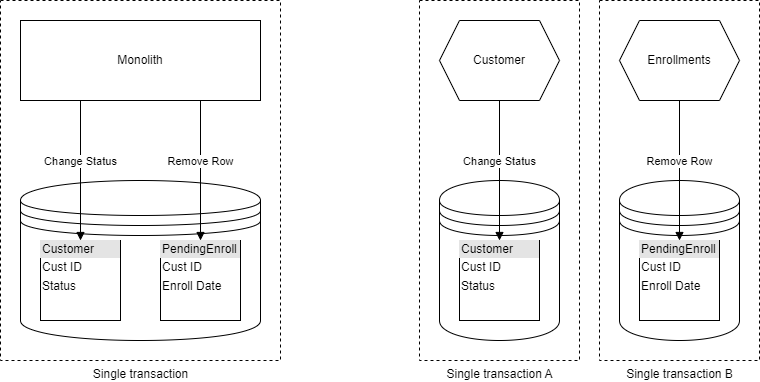
\includegraphics[scale=0.5]{Pictures/3_transaction.png}
    \caption{Example that show the difference between monolithic and microservices transactions.}
    \label{fig:3_transaction}
\end{figure}

\subsubsection{Distributed transaction}

\subsubsection{SAGAS Pattern}
% sagas (something I’ll detail at length in Chapter 6)

\section{Serverless}
\subsection{Event-driven design}

\section{Technologies}
\subsection{Amazon AWS Services}
% https://aws.amazon.com/what-is-aws/
AWS is recognized as the world's most comprehensive and broadly adopted cloud platform. It offers
over 175 fully featured services from data centers globally. AWS is utilized by a diverse range of
customers, including rapidly growing startups, large enterprises, and leading government agencies,
to reduce costs, increase agility, and accelerate innovation. The platform provides a wide array of
cloud-based products including compute, storage, databases, analytics, networking, mobile, developer
tools, management tools, IoT, security, and enterprise applications, all available on-demand with
pay-as-you-go pricing.
\subsubsection{AWS API Gateway}
\subsubsection{AWS Lambda}
\subsubsection{AWS RDS}
\subsubsection{AWS SQS}
\subsubsection{AWS SNS}
\subsection{Firebase}
\subsection{GO Language}
\subsubsection{GO CDK}
\subsubsection{GORM}
\subsection{Serverless framework}
\subsection{Flutter}
